\documentclass[]{beamer}
\mode<presentation>
{
  \usetheme{Warsaw}
  \definecolor{mcgarnet}{rgb}{0.38, 0, 0.08}
  \definecolor{mcgray}{rgb}{0.6, 0.6, 0.6}
  \setbeamercolor{structure}{fg=mcgarnet,bg=mcgray}
  %\setbeamercovered{transparent}
}


\usepackage[english]{babel}
\usepackage[latin1]{inputenc}
\usepackage{times}
\usepackage[T1]{fontenc}
\usepackage{tikz}
\usepackage{graphicx}
\usepackage{fancyvrb}
\usepackage{adjustbox}

\newcommand{\imagesource}[1]{{\centering\hfill\break\hbox{\scriptsize Image Source:\thinspace{\small\itshape #1}}\par}}

\title{09 - Going Loopy - Part 2}


\author{Dr. Robert Lowe\\}

\institute[Maryville College] % (optional, but mostly needed)
{
  Division of Mathematics and Computer Science\\
  Maryville College
}

\date[]{}
\subject{}

\pgfdeclareimage[height=0.5cm]{university-logo}{images/Maryville-College}
\logo{\pgfuseimage{university-logo}}



\AtBeginSection[]
{
  \begin{frame}<beamer>{Outline}
    \tableofcontents[currentsection]
  \end{frame}
}


\begin{document}

\begin{frame}
  \titlepage
\end{frame}

\begin{frame}{Outline}
  \tableofcontents
\end{frame}


% Structuring a talk is a difficult task and the following structure
% may not be suitable. Here are some rules that apply for this
% solution: 

% - Exactly two or three sections (other than the summary).
% - At *most* three subsections per section.
% - Talk about 30s to 2min per frame. So there should be between about
%   15 and 30 frames, all told.

% - A conference audience is likely to know very little of what you
%   are going to talk about. So *simplify*!
% - In a 20min talk, getting the main ideas across is hard
%   enough. Leave out details, even if it means being less precise than
%   you think necessary.
% - If you omit details that are vital to the proof/implementation,
%   just say so once. Everybody will be happy with that.

\section{A Common Pattern}

\begin{frame}[fragile]{A Common Type of Loop}
\begin{columns}
    \column{0.6\textwidth}
    \begin{block}{Basic Counting Loop}<2->
    \textit{initialize}
    \newline\verb!while(!\textit{condition}\verb!) {!
    \newline\verb!    !\textit{loop body}
    \newline\verb!    !\textit{update}
    \newline\verb!}!
    \end{block}
   
    \begin{block}{Example: Count to 10}<3->
    \verb!num = 0;!
    \newline\verb!while(num <= 10) {!
    \newline\verb!    cout << num << endl;!
    \newline\verb!    num++;!
    \newline\verb!}!
    \end{block}

    \column{0.4\textwidth}
    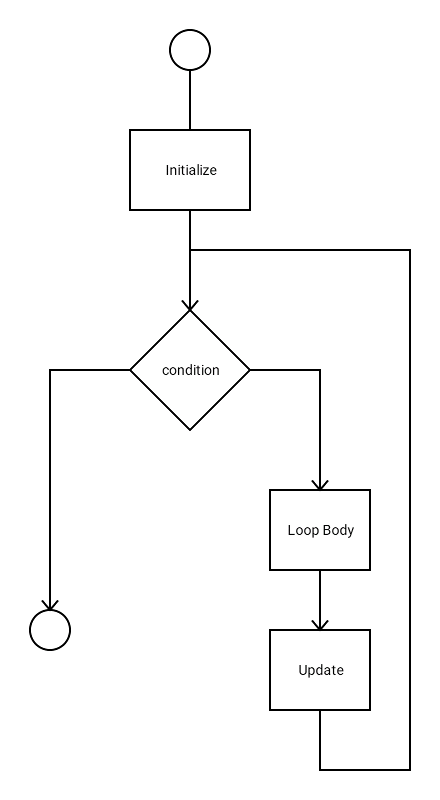
\includegraphics[width=0.9\textwidth]{images/for}
\end{columns}
\end{frame}

\begin{frame}[fragile]{\texttt{for}: A Convenient Pre-Test Loop Format}
\begin{columns}
    \column{0.6\textwidth}
    \begin{block}{The For Loop}<2->
        \verb!for(! \textit{initialize}; \textit{condition}; \textit{update}\verb!) {!
        \newline\verb!    !\textit{loop body}
        \newline\verb!}!
    \end{block}

    \begin{block}{Example: Count to 10}<3->
        \verb!for(num=0; num <= 10; num++)!
        \newline\verb!{!
        \newline\verb!    cout << num << endl;!
        \newline\verb!}!
    \end{block}

    \column{0.4\textwidth}
    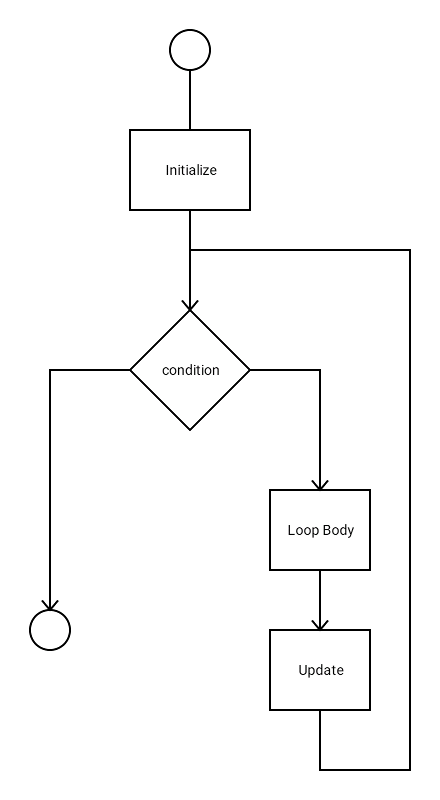
\includegraphics[width=0.9\textwidth]{images/for}
\end{columns}
\end{frame}

\begin{frame}[fragile]{Declaring Variables During Loop Initialization}
    \begin{itemize}[<+->]
        \item If a variable is only used within the loop, it is
            customary to declare it in the \texttt{for} loop's
            initializer.
        \item Take, for example, the main function of
            \texttt{examples/09-Loopy/count.cpp}.
            \begin{verbatim}
int main()
{
    //count to 10
    for(int num=0; num <= 10; num++) {
        //display the number
        cout << num << endl;
    }
}
            \end{verbatim}
        \item Note that when you do this, the variable is
            \textbf{only} available in the \texttt{for} loop.
    \end{itemize}
\end{frame}

\begin{frame}{Dr. Lowe's Guide to Loop Selection}
    \begin{itemize}[<+->]
        \item Use a \texttt{\textbf{for}} loop when:
            \begin{itemize}
                \item You are counting.
                \item You have a fixed number of iterations.
                \item You are exploring the entire contents of a list.
            \end{itemize}
        \item Use a \texttt{\textbf{while}} loop when:
            \begin{itemize}
                \item You are scanning for some sentinel data.
                \item You are reading to the end of input.
                \item You are waiting for some general condition to be
                    met.
            \end{itemize}
        \item Use a \texttt{\textbf{do..while}} loop when:
            \begin{itemize}
                \item You are validating user input.
                \item You are building a menu interface.
                \item You need to go through a loop at least one time.
            \end{itemize}
    \end{itemize}
\end{frame}

\begin{frame}[fragile]{Converting a \texttt{while} Loop to a For Loop}
\begin{columns}
    \column{0.4\textwidth}
    \begin{adjustbox}{max width=\textwidth}
    \begin{BVerbatim}
int num;

//initialize
num = 0;

//count to 10
while(num <= 10) {
    //display the number
    cout << num << endl;

    //increment
    num++;
}
    \end{BVerbatim}
    \end{adjustbox}

    \column{0.6\textwidth}
    \begin{adjustbox}{max width=\textwidth}
    \begin{BVerbatim}
//count to 10
for(int num=0; num <= 10; num++) {
    //display the number
    cout << num << endl;
}
    \end{BVerbatim}
    \end{adjustbox}
\end{columns}
\end{frame}

\begin{frame}{\textbf{Lab Activity:} Convert to For Loops}
    \begin{enumerate}
        \item Create the directory \texttt{labs/week6}
        \item Copy the following files from \texttt{labs/week4} to
            \texttt{labs/week6}.
            \begin{itemize}
                \item \texttt{count2.cpp}
                \item \texttt{fahrenheit.cpp}
            \end{itemize}
        \item Convert the loops in these programs to \texttt{for}
            loops.
        \item Compile and test your programs.
    \end{enumerate}
\end{frame}

\section{Some Common Pitfalls}

\begin{frame}[fragile]{Incrementing Twice}
    \begin{itemize}[<+->]
        \item One common mistake to make with \texttt{for} loops is to
            increment your counting variable twice.
        \item For instance, consider the following:
        \begin{BVerbatim}
    //count to 10
    for(int num=0; num <= 10; num++) {
        //display the number
        cout << num << endl;

        //update the number
        num++;
    }
        \end{BVerbatim}
        \item Fixing this is pretty easy, just remove the extra
        update!
    \end{itemize}
\end{frame}

\begin{frame}[fragile]{On the Dangers of Doubles}
    \begin{itemize}[<+->]
        \item Change into the \texttt{examples/09-Loopy} directory.
        \item Compile and run the \texttt{double-count.cpp} example.
        \item This program should count from 0 to the specified
            \texttt{double} using a given number of lines, each
            consisting of 4 columns (counting down each column).
        \item Consider the following sample run:
\begin{BVerbatim}
What should I count to? 1.0
How many lines? 2
0.0000  0.2857  0.5714  0.8571  
0.1429  0.4286  0.7143  1.0000
\end{BVerbatim}
        \item Play around with this a bit. Does it always work?
        \item No!  This is because of the imprecision in
            \texttt{double} calculations and comparison!
    \end{itemize}
\end{frame}

\begin{frame}[fragile]{Best Practices for Loops With Doubles}
    \begin{itemize}[<+->]
        \item We should generally avoid using \texttt{double}
            variables to perform counting.
        \item If we want to iterate through doubles, we should instead
            count using an \texttt{int}. 
        \item Calculate the double within the loop.
        \item This is often done using the comma operator to do two
            calculations in the update:
            \newline\verb#line++, start += increment#
    \end{itemize}
\end{frame}

\begin{frame}[fragile]{Lab Activity: Repair \texttt{double-count.cpp}}
    \begin{enumerate}
        \item Copy \texttt{examples/09-Loopy/double-count.cpp} to
            \texttt{labs/week6}.
        \item Repair the loop by changing it to this:
        \begin{adjustbox}{max width=0.9\textwidth}
        \begin{BVerbatim}
    //Go through each row
    double start=0.0;
    for(int line=0; line < lines;  line++, start += increment) {
        //find max for this row
        double row_max = start + 3.0 * lines * increment; 

        if(row_max <= max) {
            //print all the columns
            double num=start;
            for(int col=0; col<4; col++, num+=lines * increment){
                cout << num << "\t";
            }
            cout << endl;
        }
    }
        \end{BVerbatim}
        \end{adjustbox}
    \end{enumerate}
\end{frame}

\begin{frame}{Infinite Loops and Other Pitfalls}
    \begin{itemize}[<+->]
        \item Another common mistake is to forget to change a loop
            variable.  This will cause an infinite loop.
        \item Misplaced semicolons are also a common way to mistakenly
            generate an infinite loop.
            \newline\texttt{while(x<=5); \{}
        \item Off by one errors are also a common mistake!
        \item Be careful about \texttt{<} vs \texttt{<=}, and be sure
            to select the correct one!
    \end{itemize}
\end{frame}


\end{document}


